\section{Parallel Architectures}

\textbf{Flynn's Taxonomy}
\begin{itemize}
    \item Single Instruction (SI) - System in which all processors execute the same instruction
    \item Multiple Instruction (MI) - System in which different processors execute different instructions
    \item Single Data (SD) - System in which all processors operate on the same data
    \item Multiple Dara (MD) - System in which different processors may operate on different data.
\end{itemize}

\begin{itemize}
    \item SISD - Classic von Neumann architecture; serial computer
    \item MIMD - Collection of autonomous processors that can execute multiple independent programs; each of which can have its own data stream
    \item SIMD - Data is devided among the processors and each data item is subjected to the same sequnce of instructions; GPUs; Advanced Vector Extensions (AVX)
    \item  MISD - Very rare;
\end{itemize}

\textbf{MIMD Architectures (Shared Memory)} \par

\textbf{Uniform Memory Access (UMA)} - Each cpu uses same memory. \par

\textbf{Non-Uniform Memory Access (NUMA)} - Each set of CPU uses a part of the memory. \par

\textbf{Distributed Memory} \par

\textbf{Hybrid Memory} \par 

\section{Performance}

\textbf{Efficacy} - Computational requirements (what needs to be done?) \par
\textbf{Efficiency} - Computing resources (how much will it cost?) \par

\textbf{Embarrassingly Parallel Computation} - is one that can be obviously divided into completely independent parts that can be executed simultaneously. (Trully - there is no interaction, nearly - result must be collected in some way)

\section{Performance Metrics and Formulas}

$S(p) = \frac{T_1}{T_p}$ , $E(p) = \frac{S_p}{p , Cost(p) = p * T_p}$

\section{Amddahl's Law}

Interested in solving problems faster.\par

- Time: wall clock time

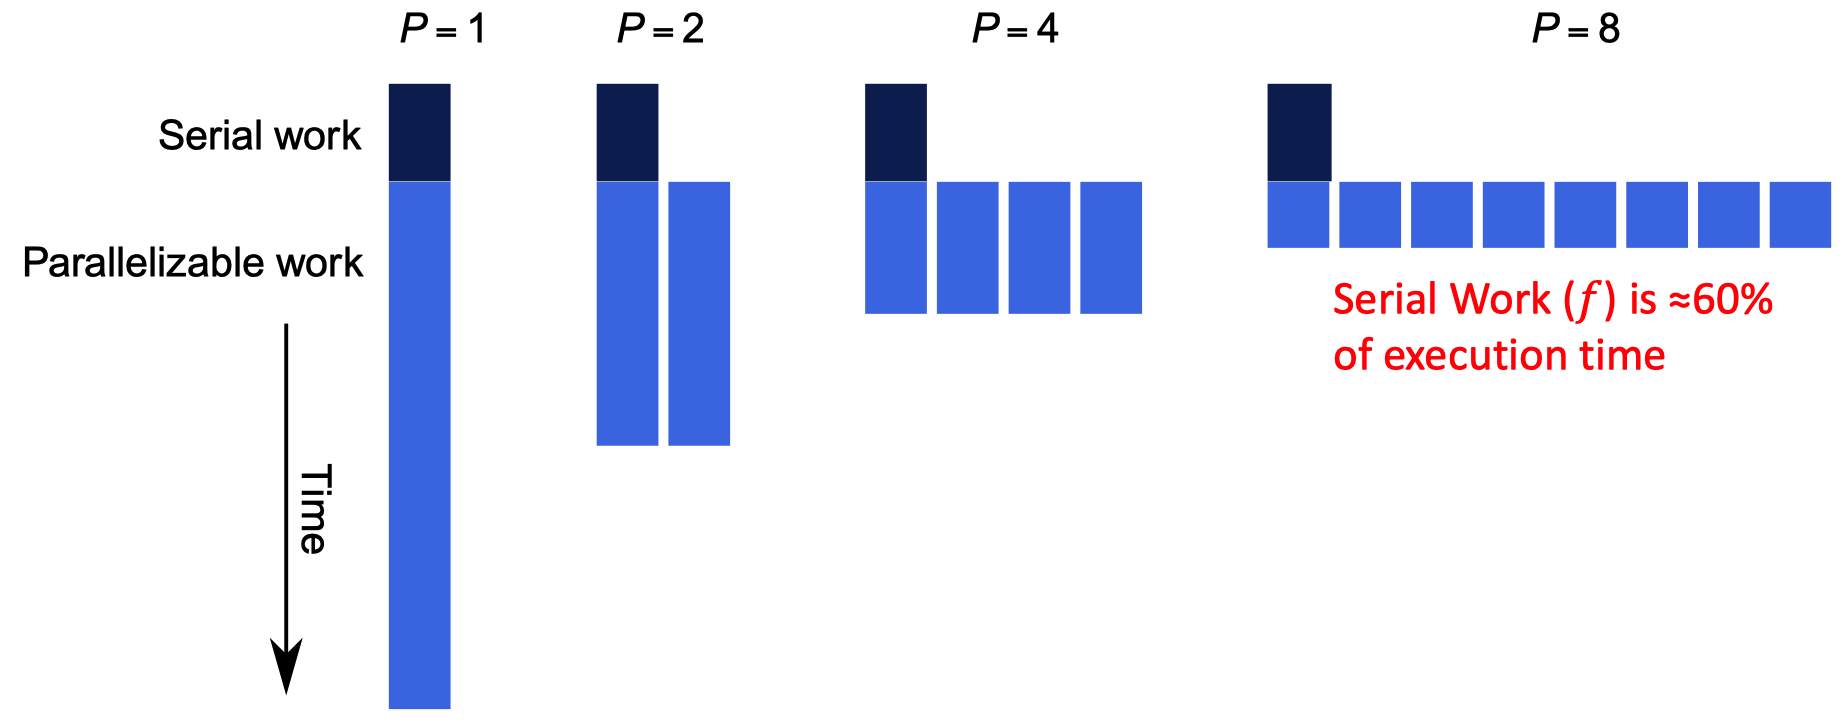
\includegraphics[width=\linewidth]{img/Amh.png}

$S_p <= \frac{1}{f + \frac{(1-f)}{p}}$, $S_{p->inf} <= \frac{1}{f}$ \par

\section{Gustafson-Barsis Law}

- Often interested in large problems when scaling\par
- Time: CPU time

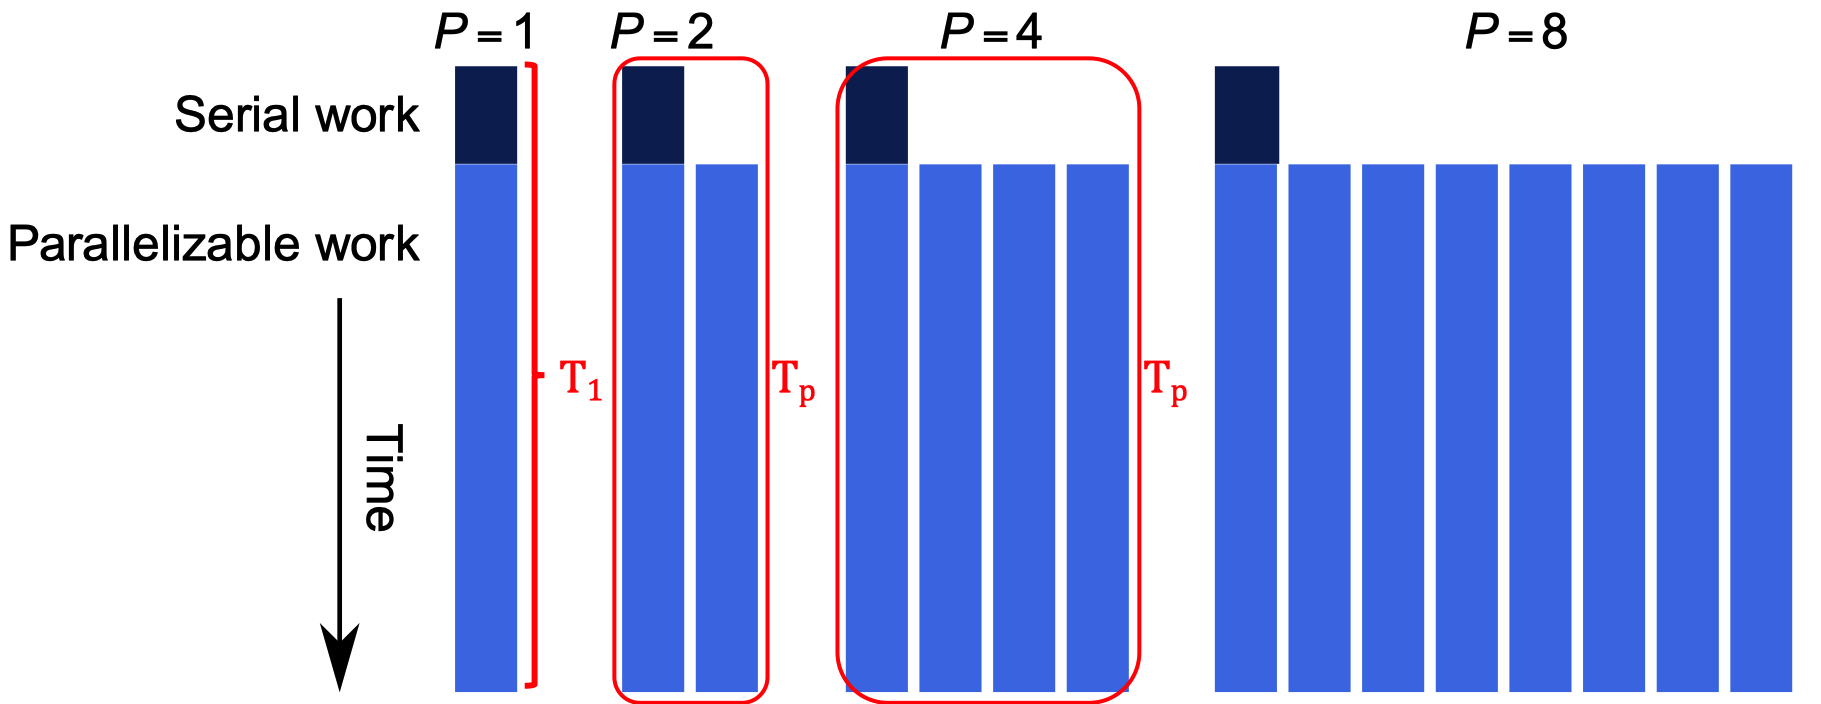
\includegraphics[width=\linewidth]{img/gus.png}

$S <= \alpha + P.(1  - \alpha)$

\subsection{Work-Span}

\textbf{Work Law:} $T_p \geq \frac{T_1}{P}$ \par
\textbf{Span Law:} $T_p \geq T_\infty$\par

\textbf{Speedup} = $\frac{T_1}{T_p}$ on P Processors \par

If $T_1/T_p = P,$we have (perfect) linear speedup.\par

If $T1/Tp > P$, we have superlinear speedup, which is not possible in this performance model, beacuse of the work Law.\par

We can write a work-span formula to derive a lower bound on $T_p$ : $Max(T_1/P,T_\infty) \leq T_p $ \par

Brent's Lemma derives an upper bound: Captures the additional cost executing the other tasks not on the critical path, assume can do so without overhead.\par

$T_p \leq (T_1 - T_\infty) / P + T_\infty$